\documentclass[conference]{IEEEtran}
\IEEEoverridecommandlockouts
%Template version as of 6/27/2024

\usepackage{cite}
\usepackage{amsmath,amssymb,amsfonts}
\usepackage{algorithmic}
\usepackage{graphicx}
\usepackage{textcomp}
\usepackage{xcolor}
\def\BibTeX{{\rm B\kern-.05em{\sc i\kern-.025em b}\kern-.08em
    T\kern-.1667em\lower.7ex\hbox{E}\kern-.125emX}}

\begin{document}

\title{Detection of Potential Depressive Disorders on ``X'' Social Media Based on User-Level Analysis Using Multi-Modal Transformers Architecture}

\author{
\IEEEauthorblockN{\small Mohammad Arkananta Radithya Taratugang}
\IEEEauthorblockA{\textit{Department of Information Technology}\\
\textit{Institut Teknologi Sepuluh Nopember}\\
Surabaya, Indonesia\\
5027221003@student.its.ac.id}
\and
\IEEEauthorblockN{\small Hafara Firdausi}
\IEEEauthorblockA{\textit{Department of Information Technology}\\
\textit{Institut Teknologi Sepuluh Nopember}\\
Surabaya, Indonesia\\
hafara@its.ac.id}
\and
\IEEEauthorblockN{\small Annisaa Sri Indrawanti}
\IEEEauthorblockA{\textit{Department of Information Technology}\\
\textit{Institut Teknologi Sepuluh Nopember}\\
Surabaya, Indonesia\\
annisaa@its.ac.id}
}

\maketitle

% ---------------------------------------------------------------
\begin{abstract}
\textit{Existing automated depression detection systems on social media are
often limited to post-level analysis, failing to capture chronic
emotional patterns. This study develops a user-level depression
identification system on the ``X'' platform based on DSM-5 clinical
criteria. A Multimodal Transformer architecture was developed by
fine-tuning IndoBERTweet for text and Vision Transformer (ViT) for
image feature extraction. The model analyzes users' timeline histories
to distinguish situational negative emotions from consistent clinical
indications. Transparency is ensured through Explainable AI (XAI)
attention maps. Implemented as a browser extension, the system
aggregates 50-100 recent posts for hybrid scoring. Experimental
results show the Multimodal ViT fusion achieves 82.10\% accuracy and
79.10\% F1-Score. Although the performance increase over the text-only
model is not statistically significant, the multimodal fusion reduces
false-negatives to the lowest observed count (13 vs.\ 16 for ResNet-18), a
clinically critical advantage. Clinical psychologist validation
confirmed alignment with medical reasoning and ethical output
terminology (``Stress Indication''). Furthermore, End-User Testing
yielded a System Usability Scale (SUS) score of 80, proving its
feasibility as a proactive, user-friendly early screening instrument.
These findings demonstrate that integrating multimodal deep learning with
explainable AI presents a promising, ethically responsible decision-support
tool for preliminary mental health screening. By prioritizing high recall, 
the system serves as a practical screening aid to facilitate 
proactive mental health outreach in digitized environments.}
\end{abstract}

\renewcommand\IEEEkeywordsname{Keywords}
\begin{IEEEkeywords}
Depression, IndoBERTweet, Social Media X, Explainable AI,
Vision Transformer, DSM-5, Browser Extension.
\end{IEEEkeywords}

% ---------------------------------------------------------------
\section{Introduction}

The rapid growth in the use of social media such as X (formerly
Twitter) has fundamentally changed the global communication landscape,
allowing users to express their thoughts, feelings, and emotional
states instantly. The X platform remains one of the primary spaces
frequently used by individuals to pour their hearts out
(\emph{self-disclosure}) anonymously, indirectly recording the digital
footprint of their mental health conditions \cite{b_dhinora}.

Mental health, particularly depressive disorders, has become a crucial
issue requiring immediate attention globally and specifically in Indonesia. According to the World Health Organization (WHO), depression is a leading cause of disability worldwide, affecting over 280 million people \cite{b_who}. In the context of Indonesia, the Ministry of Health reports a significant surge in depressive symptoms among adolescents and young adults (Gen Z), heavily correlated with the post-pandemic digital lifestyle. Based on the clinical
criteria in the \emph{Diagnostic and Statistical Manual of Mental
Disorders} (DSM-5), major depression is characterized by persistent
symptoms such as depressed affect, constant loss of energy, and
anhedonia, which adversely impact social functioning \cite{b_apa}. The DSM-5 explicitly notes that a diagnosis requires these symptoms to be present for a minimum of two weeks, emphasizing the critical need for temporal, long-term observation rather than isolated assessments.
Although the urgency is real and its prevalence continues to rise,
many depression sufferers are reluctant to seek professional help,
primarily because of social stigma and limited access to psychological facilities \cite{b_anastasia}.

These conditions drive sufferers to prefer expressing their despair
through social media posts using unique language patterns.
Psycholinguistic research shows that depression sufferers tend to use
absolutist words \cite{b_almosaiwi} and an increased intensity of
first-person singular pronouns \cite{b_eichstaedt}. Preemptive
detection through social media analysis can provide opportunities for
earlier clinical intervention \cite{b_owen}.

However, the main challenge is the highly informal nature of social
media language. In Indonesia, X users dominate the timeline with
slang, non-standard abbreviations, code-mixing, and metaphorical
expressions \cite{b_koto}. Furthermore, accurate depression detection
must be conducted by collectively analyzing the user's entire posting
history (\emph{user-level analysis}) to distinguish situational
sadness from chronic depressive episodes \cite{b_alasad, b_zogan}.
Existing multimodal studies largely ignore user-level temporal
patterns, limiting their applicability to real-world early detection
scenarios.

Another limitation is that conventional models often rely solely on
text. In reality, users frequently post images that reinforce emotional
intensity \cite{b_faiz}. Unimodal analysis is prone to diagnostic
errors when sentence meaning heavily depends on accompanying visual
context.

Based on this background, this study designs an intelligent system for
detecting potential depression at the user level using a Multimodal
Transformers architecture. IndoBERTweet is combined with the Vision
Transformer (ViT) using late fusion to process complex
text-image relations. An Explainable AI (XAI) mechanism is also
integrated to visualize the reasoning behind each decision, ensuring
clinically transparent and accountable results.

% ---------------------------------------------------------------
\section{Literature Review}

The X platform encourages open self-disclosure. The linguistic
expression of depression sufferers is often characterized by high
usage of first-person singular pronouns \cite{b_eichstaedt} and
absolutist words (e.g., always, never) indicating dichotomous thinking
\cite{b_almosaiwi}. In the Indonesian context, these expressions
predominantly use non-standard language, abbreviations, and
code-mixing \cite{b_koto}.

Previous studies attempted to solve this challenge through various
approaches. Al~Asad et al.\ \cite{b_alasad} proposed user-level
analysis but did not integrate visual modality. Zogan et al.\
\cite{b_zogan} combined textual and behavioral features to improve
accuracy, yet their model remains text-only. Willie et al.\
\cite{b_willie} highlighted the urgency of domain-specific language
models, though they did not address the Indonesian slang context.
These text-only approaches exhibit a critical vulnerability when analyzing modern social media behavior, where depressive affect is frequently masked by sarcastic text or juxtaposed against contradictory imagery. A unimodal text system processing a user's self-deprecating meme would invariably misclassify it as non-depressive due to the absence of explicit distress vocabulary. Therefore, integrating a visual modality is no longer an optional enhancement but a theoretical necessity to capture the holistic emotional state of the user.

The Transformers architecture \cite{b_vaswani}, which fundamentally revolutionized natural language processing by dispensing with recurrence and convolutions, relies entirely on a sophisticated attention mechanism. This architecture evolved into
BERT \cite{b_devlin}, which gave rise to IndoBERTweet, a domain-specific model trained on
409 million Indonesian tweets. Its Scaled Dot-Product Attention
allows simultaneous computation of relational weights across words, capturing long-range dependencies and bidirectional context. This capability makes it the new gold standard for understanding the highly nuanced and informal Indonesian
text on the X platform \cite{b_koto}.

To address the visual modality, the Vision Transformer (ViT) adapts the same self-attention mechanism
for computer vision by dividing images into a sequence of non-overlapping
fixed-size patches ($P \times P$) \cite{b_dosovitskiy}. By treating these patches similarly to tokens in NLP, ViT applies Positional
Embedding to preserve the spatial understanding of objects. This purely self-attentional approach to images has
proven highly robust, particularly when aligned with Transformer-based text models
in cross-modal learning scenarios \cite{b_radford}. 

In multimodal systems, the fusion strategy dictates how different modalities interact. The late fusion strategy, fundamentally based on feature
concatenation at the decision level \cite{b_kiela}, allows the text (IndoBERTweet) and image (ViT)
encoders to operate independently and optimize their distinct modality-specific weights. Their respective 768-dimensional outputs
are concatenated into a highly expressive 1536-dimensional multimodal vector. This approach avoids the
feature distortion and overwhelming computational complexity that are highly prone to occur in early or mid-level fusion architectures \cite{b_lu}.

An Explainable AI (XAI) module is implemented to visualize Attention
Maps and dominant keyword contributions \cite{b_vig}. SHAP
(SHapley Additive exPlanations) is crucial for opening the
``black-box'' of deep learning \cite{b_lan}, providing transparent
empirical evidence that clinical psychologists can verify.

% ---------------------------------------------------------------
\section{Methodology}

The overall system workflow is illustrated in Fig.~\ref{fig:flow}.

\begin{figure}[!ht]
\centerline{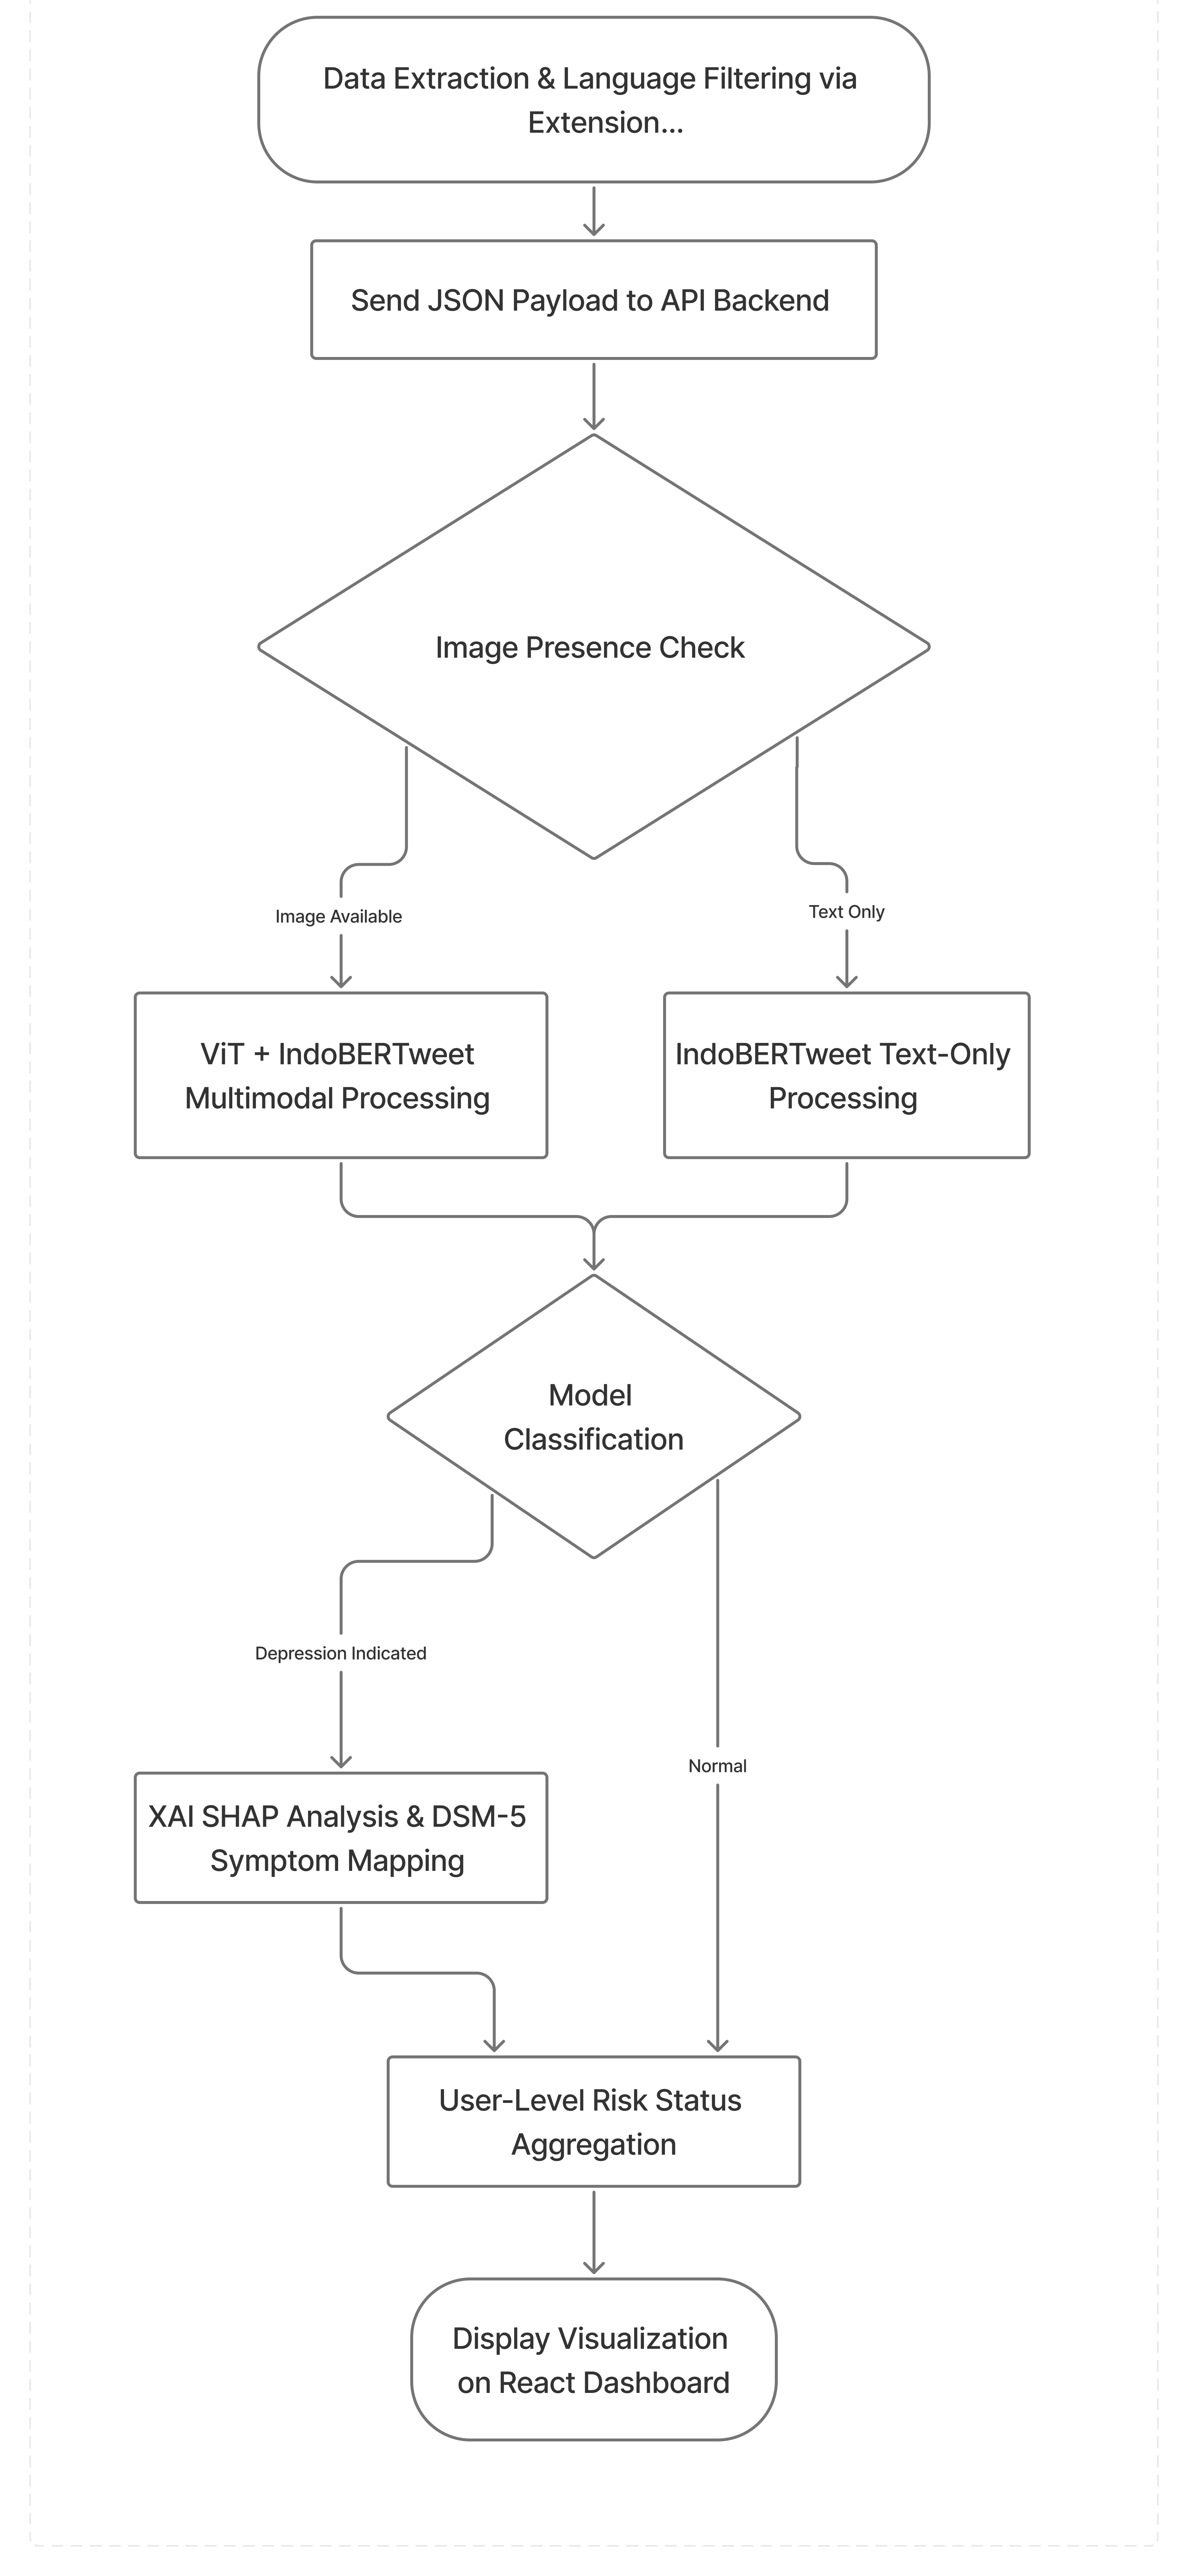
\includegraphics[width=0.86\linewidth]{systemflow.png}}
\caption{System flowchart.}
\label{fig:flow}
\end{figure}

\subsection{Data Collection and Inter-Rater Reliability (Gwet's AC1)}
Data collection employed a dual-source strategy. The textual corpus originates from a public Indonesian Twitter dataset (6,982 raw tweets), augmented via the \emph{llama-3.3-70b-versatile} LLM using tailored prompts to generate Gen~Z slang variations and contextual depressive metaphors. To resolve class imbalance, dynamic undersampling was applied to the majority Normal class to match the expanded Depressive instances, yielding a strictly balanced benchmark corpus of 7,991 text samples (50\% depressive, 50\% normal). The corpus was partitioned with a 70/15/15 ratio into 70\% training (5,593 samples), 15\% validation (1,199 samples), and an independent 15\% test set (1,199 samples). To prevent lexical data leakage, group-based splitting ensured that original tweets and their LLM paraphrased variations were strictly bound to the same partition and never crossed into the test split.

In parallel, a multimodal dataset comprising 294 organic tweet-image pairs was collected in real-time via Selenium WebDriver, filtered for Indonesian personal self-disclosures. To eliminate user-level identity and writing-style leakage, data points were sampled across distinct, non-overlapping user timelines (user-disjoint sampling). Three psychology student annotators independently labeled the multimodal corpus. Inter-Rater Reliability was measured using Gwet's AC1 \cite{b_gwet} to avoid high-agreement paradoxes common to Cohen's Kappa, formulated as:
\begin{equation}
AC1 = \frac{p_a - p_{e(\gamma)}}{1 - p_{e(\gamma)}}
\end{equation}
where $p_a$ represents overall percent agreement and $p_{e(\gamma)}$ is the chance-agreement probability adjusted for marginal distributions. Across 195 overlapping cross-annotated instances, the evaluation yielded an $AC1$ score of 0.8558, demonstrating ``Almost Perfect Agreement'' under Gwet's benchmark guidelines. Ambiguous labels were resolved via consensus with a licensed clinical psychologist. To respect subject privacy while maintaining raw pixel fidelity for ViT feature extraction, this organic multimodal repository is strictly held in a private research vault.


\subsection{Data Preprocessing}
Text preprocessing for IndoBERTweet includes Data Cleansing (removing
URLs, hashtags, mentions), Case Folding to lowercase, and Tokenization
using the built-in IndoBERTweet tokenizer. Image preprocessing for
ViT includes Resizing to $224 \times 224$ pixels, Normalization of
pixel intensity, and Image Patching into $16 \times 16$ pixel patches.

\subsection{Multimodal Transformer Architecture}
The proposed architecture integrates the pre-trained IndoBERTweet
\cite{b_koto} to extract text features (768-dimensional vector) and
ViT to extract image features. The combination is carried out through
Late Fusion (feature concatenation) \cite{b_kiela}, producing a
1536-dimensional combined vector $v_{fusion}$:
\begin{equation}
v_{fusion} = [v_{text} \oplus v_{image}], \quad v_{fusion} \in \mathbb{R}^{1536}
\end{equation}
where $\oplus$ denotes the concatenation operator. A Dynamic Routing mechanism
automatically switches to text-only fallback mode if no image is
detected, ensuring lightweight inference.

\begin{figure}[!ht]
\centerline{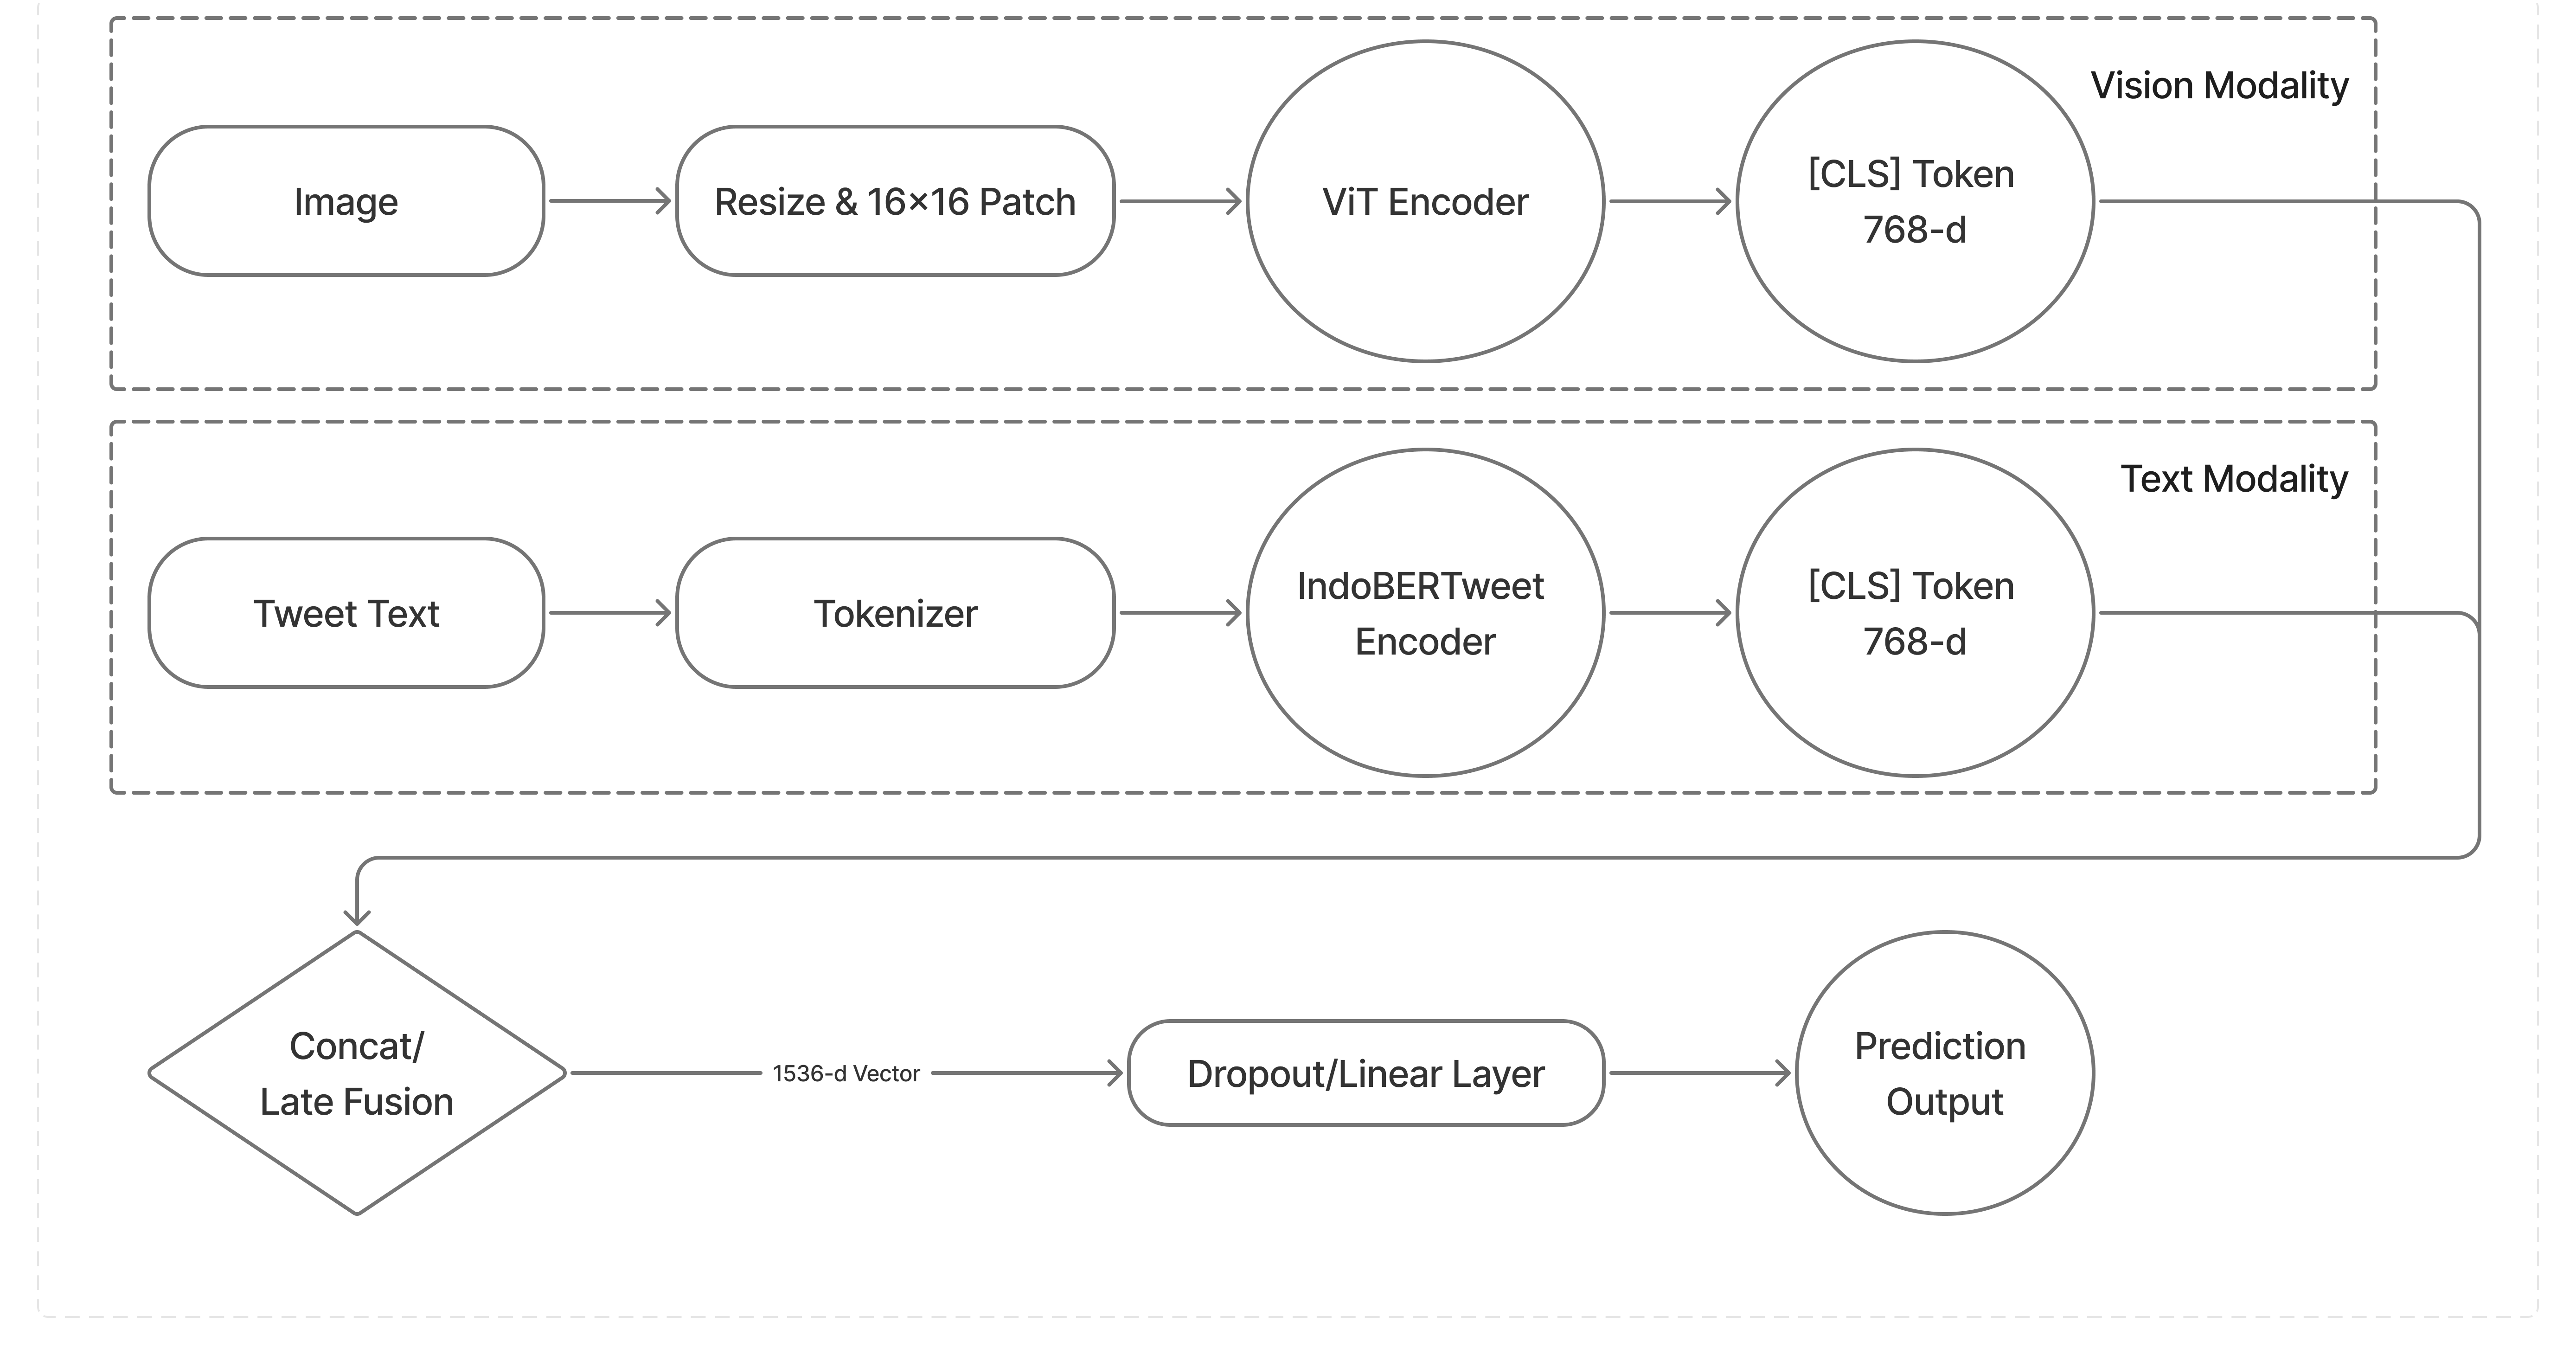
\includegraphics[width=1.03\linewidth]{modelarchitecture.png}}
\caption{Multimodal Late Fusion Architecture.}
\label{fig:arsitektur}
\end{figure}

\subsection{Recall-Priority Training Strategy}
To minimize False Negatives, the training strategy prioritized Recall
as the primary model selection metric via
\texttt{metric\_for\_best\_model=``recall''} in the HuggingFace
\texttt{Trainer}. Additionally, the sentence-level classification
threshold was lowered from 0.50 to 0.25, so that any tweet with a
depression confidence score above 25\% is flagged as an indication.
The fine-tuning ran for 3 epochs (IndoBERTweet) with a batch size of
16, learning rate $2 \times 10^{-5}$, and weight decay 0.01. All computational experiments and model training were conducted in a Python 3.10 environment utilizing the PyTorch framework and HuggingFace Transformers library. Hardware acceleration was provided by an NVIDIA T4 Tensor Core GPU with 16GB of VRAM, ensuring optimal matrix multiplication performance for the high-dimensional attention layers.

\subsection{User-Level Hybrid Scoring Mechanism}
While the deep learning models operate as the core post-level affective feature extractors, psychiatric diagnosis under DSM-5 guidelines mandates evaluating persistent emotional patterns across time rather than isolated posts. To bridge post-level inference into user-level screening, the system aggregates the chronological timeline history of 50--100 recent posts within a 14-day sliding window. Risk severity is calculated using the Hybrid Scoring method \cite{b_coppersmith, b_uban}, determining the final user-level risk score ($R$) by combining the global average confidence ($S_{global}$) and the peak average score ($S_{peak}$):
\begin{equation}
R = (0.4 \times S_{global}) + (0.6 \times S_{peak})
\end{equation}
This formulation emphasizes acute depressive episodes while maintaining the context of longitudinal mood consistency. The aggregated user risk ($R$) is categorized into High Potential ($>$30\%), Moderate (15\%--30\%), and Stable ($<$15\%).

\subsection{Dashboard Implementation and Semantic Mapping (SBERT)}
The final implementation is packaged within a Client-Server
architecture: a browser extension for passive real-time scanning and
DOM extraction, and a FastAPI backend. The system implements
Indo-SBERT (Sentence-BERT) to extract semantic vectors from tweets
and calculate Cosine Similarity against the nine main DSM-5 criteria.
The semantic alignment score for each post $d$ against DSM-5 criterion
$c_i$ is computed as:
\begin{equation}
\text{sim}(d, c_i) = \frac{\vec{v}_d \cdot \vec{v}_{c_i}}{\|\vec{v}_d\| \, \|\vec{v}_{c_i}\|}
\end{equation}
where $\vec{v}_d$ and $\vec{v}_{c_i}$ are the SBERT embedding vectors
for the tweet and the DSM-5 criterion respectively. A post is flagged
as aligned with a criterion if $\text{sim}(d, c_i) > 0.35$. The system
counts the number of distinct DSM-5 criteria triggered across the
monitoring window, providing a structured clinical evidence trail
for each flagged user. A React-based dashboard presents chronological
emotional trend visualizations over a 14-day window, text highlighting,
and early intervention recommendations \cite{b_apa}.

% ---------------------------------------------------------------
\section{Results and Discussion}

\subsection{Text Classification Model Testing Results}
The pre-trained IndoBERTweet model was compared with standard IndoBERT
and BiLSTM on an independent test set (15\% of the data corpus).
BiLSTM experienced extreme difficulty mapping implicit semantics, yielding
an Accuracy of 83.46\% and a concerningly low Recall of 69.20\%,
despite a paradoxically high Precision of 97.95\%. This discrepancy
is characteristic of a precision-recall tradeoff under class imbalance:
the BiLSTM learned to predict the majority class (Normal) with high
confidence, resulting in high Precision but catastrophically missing
a large portion of true depressive cases (low Recall). The sequential
nature of the BiLSTM architecture fundamentally struggled to capture
the long-range dependencies and inverted syntax commonly found in
Indonesian social media slang. When users expressed depressive thoughts
using fragmented sentences or abruptly shifted context midway through
a tweet, the BiLSTM's memory gates often discarded critical early
context. Conversely, the self-attention mechanism within Transformer-based
architectures successfully overcame this limitation by computing global word relations simultaneously.
Although standard IndoBERT recorded slightly higher baseline metrics, qualitative analysis
revealed this over-performance was artificially inflated by test samples that were too
formal. IndoBERTweet proved its true robustness and superiority against complex tweets using
non-standard grammar (\emph{jujurly, capek bgt, pen nyerah}),
as illustrated in Table~\ref{tab:slang}. Detailed quantitative performance is provided in
Table~\ref{tab:text}.

\begin{table}[!ht]
\caption{Text Classification Model Performance Comparison}
\begin{center}
\begin{tabular}{|l|c|c|c|c|}
\hline
\textbf{Model} & \textbf{Acc} & \textbf{Prec} & \textbf{Rec} & \textbf{F1} \\
\hline
BiLSTM               & 83.46\% & 97.95\% & 69.20\% & 81.10\% \\
IndoBERT (Standard)  & 98.33\% & 97.51\% & 99.28\% & 98.38\% \\
IndoBERTweet         & 97.77\% & 97.48\% & 98.19\% & 97.83\% \\
\hline
\end{tabular}
\label{tab:text}
\end{center}
\end{table}

\begin{figure}[!ht]
\centerline{\includegraphics[width=0.85\linewidth]{../template-paper-ieee/gambar/metrics_comparison.png}}
\caption{Performance metrics comparison of text classification models.}
\label{fig:metrics}
\end{figure}

\begin{table}[!ht]
\caption{Slang Language Detection Comparison}
\begin{center}
\begin{tabular}{|p{0.52\linewidth}|c|c|}
\hline
\textbf{Tweet Sample} & \textbf{IndoBERT} & \textbf{IndoBERTweet} \\
\hline
``jujurly gw capek bgt pen nyerah aja idup rasanya hftt'' & Normal & Indicated \\
\hline
``males bgt anjir nugas mulu kapan rebahannya wkwk'' & Normal & Normal \\
\hline
\end{tabular}
\label{tab:slang}
\end{center}
\end{table}

\subsection{Multimodal Model Testing Results}
The multimodal architecture was evaluated using 5-Fold Cross
Validation. The Multimodal ViT fusion achieved the highest Accuracy
(82.10\%) among all multimodal variants, outperforming Multimodal
ResNet-18 (81.77\%), as summarized in Table~\ref{tab:multimodal}.
For reference, the text-only baseline achieved 81.10\% Accuracy.
Crucially, ViT suppressed False Negatives
to only 13 cases (vs.\ 16 for ResNet), the absolute priority in a
psychological diagnostic system.

\begin{table}[!ht]
\caption{Multimodal Classification Comparison (5-Fold CV) (best false-negative count highlighted)}
\begin{center}
\begin{tabular}{|l|c|c|}
\hline
\textbf{Architecture} & \textbf{Accuracy} & \textbf{False Neg.} \\
\hline
Multimodal ResNet  & 81.77\% & 16  \\
\textbf{Multimodal ViT} & \textbf{82.10\%} & \textbf{13} \\
\hline
\end{tabular}
\label{tab:multimodal}
\end{center}
\end{table}

A Paired t-Test at $\alpha\,{=}\,0.05$ confirmed that the performance
increase is not statistically significant ($p > 0.05$ for all metrics,
smallest $p\,{=}\,0.345$ for Accuracy). Detailed significance test
results are in Table~\ref{tab:ttest}. This null result is expected and
attributable to three compounding factors. First, the multimodal dataset
size of only 294 samples yields insufficient statistical power to detect
small performance differences (approximately 1\%) with a paired t-Test,
a well-known limitation of small-sample clinical studies. Second, a
\emph{ceiling effect} is observed: IndoBERTweet already captures the
majority of discriminative depressive linguistic signals, leaving a
narrow margin for the visual modality to contribute additional
predictive value. Third, and most critically, images on the X platform
are inherently noisy; users frequently attach incongruent visual media
(e.g., memes, song lyrics, or random aesthetic photos) to depressive
texts, causing the ViT encoder to receive misleading rather than
complementary affective signals. This is a platform-specific limitation,
not an architectural failure. Despite the absence of statistical
significance, the multimodal fusion was retained because it is clinically
justified: minimizing False Negatives is the paramount objective in
any mental health screening system, and the ViT fusion achieved the
lowest False Negative count among all evaluated multimodal architectures.

\begin{table}[!ht]
\caption{Significance Test Results (Paired t-Test)}
\begin{center}
\begin{tabular}{|l|c|c|c|c|l|}
\hline
\textbf{Metric} & \textbf{Text} & \textbf{Multi} & \textbf{Diff} & \textbf{$p$-val} & \textbf{Sig.} \\
\hline
Acc  & 0.811 & 0.821 & +0.010 & 0.345 & No \\
Prec & 0.769 & 0.779 & +0.010 & 0.482 & No \\
Rec  & 0.818 & 0.825 & +0.007 & 0.721 & No \\
F1   & 0.781 & 0.791 & +0.010 & 0.459 & No \\
\hline
\end{tabular}
\label{tab:ttest}
\end{center}
\end{table}

\subsection{Clinical Psychologist Expert Consultation Results}
The system's clinical feasibility was evaluated through structured
Expert Consultation with a licensed Clinical Psychologist
via system demonstration and an in-depth qualitative interview. The
evaluation covered three main aspects: (1) \emph{System Functionality
Validation}, assessing the relevance of using social media digital
footprints as a psychological window and whether the analytical
dashboard output is beneficial for accelerating initial screening;
(2) \emph{Accuracy and Medical Logic Validation}, evaluating the
alignment of computational parameters with clinical psychology
standards, including risk threshold validation, XAI keyword accuracy,
DSM-5 symptom mapping, and sarcasm handling in multimodal data;
and (3) \emph{Temporal Observation and Efficiency Validation},
assessing the temporal visualization feature's ability to differentiate
reactive emotional fluctuations from persistent depression under
DSM-5 criteria, and evaluating the ethical boundaries of automated
data collection.
The expert confirmed positive results across all three dimensions.
The data fetching flow was considered reliable, and the language
criteria mapping aligns with standard clinical indicators.

The expert particularly appreciated the SHAP Partition Explainer
module for text (Fig.~\ref{fig:xai}). As validated by the expert:
\textit{``The visual explanations increase trust and the
stress-labeling avoids harmful self-diagnosis.''} As an ethical
mitigation, the system output uses the label ``Indicated'' (instead of
``Depression'') to prevent the nocebo effect of self-diagnosis. This
expert feedback confirms the qualitative feasibility of the system as
an ethical and responsible preliminary screening and decision-support aid,
rather than an autonomous diagnostic instrument.

\begin{figure}[!ht]
\centerline{\includegraphics[width=0.85\linewidth]{../template-paper-ieee/gambar/xai.png}}
\caption{SHAP attention map. The red highlighted texts represent Indonesian words that strongly influence the ``Indicated'' prediction.}
\label{fig:xai}
\end{figure}

\subsection{End-User Acceptance Testing (UAT) Results}
End-user testing adopted the System Usability Scale (SUS) instrument
\cite{b_lewis}, distributed to 14 respondents consisting of active
Gen Z users of the X platform. The system obtained an average SUS
score of 80 (SD\,=\,12.93, 95\% CI: 73-87), placing it in the
\emph{Acceptable} category with an Excellent adjective rating.
According to the SUS adjective rating scale, a score of 80 or above
is classified as Excellent, indicating a high level of user satisfaction
and learnability. This proves that the browser extension and analytical
dashboard successfully isolated the heavy computational AI complexity
on the backend while presenting a lightweight, intuitive visual
interface operable without technical assistance.

\subsection{Ethical and Privacy Considerations}
Given the sensitive nature of inferring psychological distress from personal digital footprints, several ethical safeguards and privacy preservation protocols were integrated into the system design:
\begin{itemize}
    \item \emph{Data Anonymization and Zero Retention}: All user identifiers (including @usernames, account IDs, and media URLs) are stripped during client-side DOM extraction. The FastAPI backend processes inferencing strictly in volatile memory without retaining raw user posts or personal data.
    \item \emph{Ethical Output Framing}: To prevent nocebo effects, anxiety, and inaccurate self-diagnosis, the system deliberately displays risk levels as non-diagnostic ``Stress Indications'' accompanied by prominent disclaimers rather than psychiatric verdicts.
    \item \emph{Non-Intervention and Supportive Guidance}: The system adheres to a strict non-intervention principle, operating passively without unsolicited automated messaging to analyzed accounts. Instead, structured DSM-5 symptom mapping and basic supportive guidance are provided exclusively on the dashboard as preliminary reference for clinical decision support.
\end{itemize}

% ---------------------------------------------------------------
\section{Conclusion and Suggestion}

This study successfully developed an early detection expert system for
potential depression based on Multimodal Transformers (text and
images), implemented as a browser extension. Although the Late Fusion
between IndoBERTweet and ViT achieved 82.10\% accuracy, the Paired
t-Test results proved that the image modality did not provide a
statistically significant performance improvement. Nevertheless, the
multimodal fusion was retained because it functionally suppressed
False Negatives to the lowest count among all multimodal variants
(13 cases vs.\ 16 for ResNet-18), a metric considered
extremely vital in psychological diagnostic systems.

Contextualized against related work, this study's approach offers
distinct contributions. Compared to Faiz et al.\ \cite{b_faiz}, whose
CNN-BiGRU pipeline targets post-level multimodal detection, this study
operates at the user-level by aggregating temporal tweet histories,
more closely mirroring the DSM-5 diagnostic window. Compared to Al~Asad
et al.\ \cite{b_alasad} and Zogan et al.\ \cite{b_zogan}, who
achieve user-level modeling through behavioral features alone, this
study integrates visual semantics and provides clinical-grade
transparency through XAI, a dimension absent in prior work.

This system transcended the traditional detection paradigm (post-level
analysis) toward comprehensive temporal understanding at the user level
(user-level analysis). With the Hybrid Scoring method and a 14-day
temporal monitoring window in accordance with DSM-5 guidelines, the
system effectively distinguishes fluctuating situational emotions from
consistent clinical depressive patterns. Dual validation (clinically
through Expert Judgment and by end-users via UAT, SUS\,=\,80,
Acceptable/Excellent) confirms the system is viable as an early
warning system bridge. Transparency through Explainable AI (XAI)
ensures every detection has intuitive visual accountability.

Several directions remain open for future development. At the model
level, improvements include: more precise language filtering using
FastText LangDetect to reduce code-mixing noise; an expanded
multimodal dataset with stricter sarcasm annotation protocols; and
exploration of additional visual modalities such as audio and video
from TikTok and X Spaces to capture a richer spectrum of emotional
expression.

At the system level, future work will focus on incorporating temporal
behavioral pattern signals such as active-hour distribution as an
additional depression indicator, and transitioning from browser-based
DOM extraction to the official X API for a more ethical and
non-intrusive data collection pipeline. Real-time deployment on mobile
platforms is also planned to broaden the system's clinical reach and
accessibility across diverse demographic groups.

% ---------------------------------------------------------------
\section*{Acknowledgment}
The authors gratefully acknowledge financial support from Department of Information Technology and Institut Teknologi Sepuluh Nopember for this work, under project scheme of the Publication Writing and IPR Incentive Program (PPHKI) 2025.

% ---------------------------------------------------------------
\begin{thebibliography}{00}

\bibitem{b_dhinora}
R. Dhinora et al., ``Media Sosial sebagai Medium Pengungkapan Diri di Era Digital,'' \emph{Jurnal Psikologi Siber}, 2023.

\bibitem{b_who}
World Health Organization, ``Depression: Key Facts,'' \emph{WHO}, Mar. 2023. [Online]. Available: https://www.who.int/news-room/fact-sheets/detail/depression.

\bibitem{b_apa}
American Psychiatric Association, \emph{Diagnostic and Statistical Manual of Mental Disorders (DSM-5)}, American Psychiatric Pub, 2013.

\bibitem{b_anastasia}
M. Anastasia, ``Stigma Sosial dan Keengganan Pencarian Bantuan Psikologis pada Mahasiswa,'' \emph{Jurnal Psikologi Klinis Indonesia}, 2024.

\bibitem{b_almosaiwi}
M. Al-Mosaiwi and T. Johnstone, ``In an absolute state: Elevated use of absolutist words is a marker specific to anxiety, depression, and suicidal ideation,'' \emph{Clinical Psychological Science}, vol. 6, no. 4, pp. 529-542, 2018.

\bibitem{b_eichstaedt}
J. C. Eichstaedt et al., ``Facebook language predicts depression in medical records,'' \emph{Proc. Natl. Acad. Sci.}, vol. 115, no. 42, pp. 10772-10777, 2018.

\bibitem{b_owen}
D. Owen and A. Taylor, ``Social media text analysis for early depression detection,'' \emph{IEEE Trans. Comput. Soc. Syst.}, vol. 10, no. 2, pp. 612-623, 2023.

\bibitem{b_koto}
F. Koto et al., ``IndoBERTweet: A Pretrained Language Model for Indonesian Twitter with Effective Domain-Specific Vocabulary Initialization,'' in \emph{Proc. EMNLP}, 2021.

\bibitem{b_alasad}
R. Al~Asad et al., ``User-level depression detection from social media,'' in \emph{Proc. WebSci}, 2019.

\bibitem{b_zogan}
H. Zogan et al., ``Depression Detection on Twitter using User-Level Features,'' in \emph{Proc. ACM Multimedia}, 2021.

\bibitem{b_faiz}
M. N. Faiz et al., ``Multimodal deep learning for mental disorder detection on Twitter,'' \emph{IEEE Access}, vol. 11, pp. 14520-14532, 2023.

\bibitem{b_willie}
A. Willie et al., ``Domain-Specific Language Models for Social Media Sentiment,'' in \emph{Proc. ACL}, 2020.

\bibitem{b_vaswani}
A. Vaswani et al., ``Attention is all you need,'' in \emph{Proc. NeurIPS}, 2017.

\bibitem{b_devlin}
J. Devlin et al., ``BERT: Pre-training of deep bidirectional transformers for language understanding,'' in \emph{Proc. NAACL-HLT}, 2019.

\bibitem{b_dosovitskiy}
A. Dosovitskiy et al., ``An image is worth 16x16 words: Transformers for image recognition at scale,'' in \emph{Proc. ICLR}, 2021.

\bibitem{b_radford}
A. Radford et al., ``Learning transferable visual models from natural language supervision,'' in \emph{Proc. ICML}, 2021.

\bibitem{b_kiela}
D. Kiela et al., ``Supervised Multimodal Bitransformers for Classifying Images and Text,'' in \emph{Proc. USENIX ATC}, 2019.

\bibitem{b_lu}
J. Lu et al., ``ViLBERT: Pretraining Task-Agnostic Visiolinguistic Representations for Vision-and-Language Tasks,'' in \emph{Proc. NeurIPS}, 2019.

\bibitem{b_vig}
J. Vig, ``A multiscale visualization of attention in the transformer model,'' in \emph{Proc. ACL System Demonstrations}, 2019.

\bibitem{b_lan}
M. Lan et al., ``Explainable AI for clinical decision support in mental health,'' \emph{Artificial Intelligence in Medicine}, 2024.

\bibitem{b_gwet}
K. L. Gwet, \emph{Handbook of Inter-Rater Reliability}, 2014.

\bibitem{b_coppersmith}
G. Coppersmith et al., ``Quantifying mental health signals in Twitter,'' in \emph{Proc. ACL Workshop}, 2014.

\bibitem{b_uban}
A. S. Uban et al., ``Explainable depression detection using user-level analysis,'' in \emph{Proc. CLEF}, 2021.

\bibitem{b_lewis}
J. R. Lewis, ``The system usability scale: past, present, and future,'' \emph{Int. J. Hum.-Comput. Interact.}, vol. 34, no. 7, pp. 577-590, 2018.

\end{thebibliography}

\end{document}
